\documentclass[12pt, a4paper]{article}

\usepackage{amsmath}
\usepackage{array}
\usepackage{amsmath}
\usepackage[portuguese]{babel}
\usepackage{chngpage}
\usepackage{float}
\usepackage[a4paper, margin=2cm]{geometry}
\usepackage{graphicx}
\usepackage{hyperref}
\usepackage{listings}
\usepackage{setspace}
\usepackage{xcolor}

\lstdefinestyle{codestyle}{
    commentstyle=\color{teal},
    keywordstyle=\color{blue},
    numberstyle=\ttfamily\color{gray},
    stringstyle=\color{red},
    basicstyle=\ttfamily\footnotesize,
    breakatwhitespace=false,
    breaklines=false,
    keepspaces=true,
    numbers=none,
    showspaces=false,
    showstringspaces=false,
    showtabs=false,
    tabsize=4
}
\lstset{style=codestyle}

\title{\Huge \textbf{Computação Gráfica \\ \Large Trabalho Prático -- Fase II}}
\date{30 de março 2025}
\author{Grupo 3}

\begin{document}

\begin{center}
    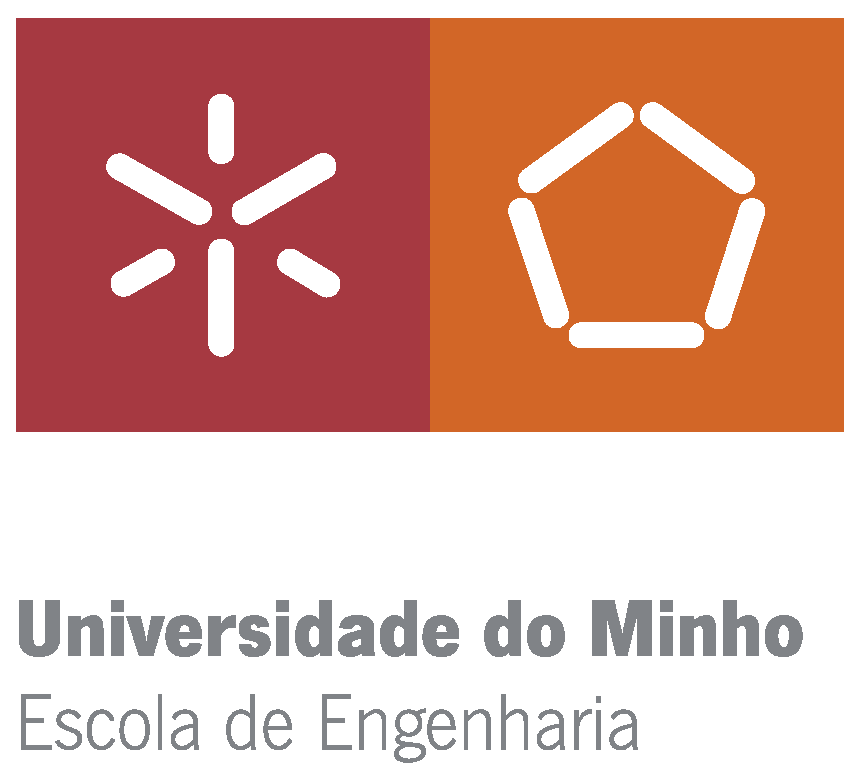
\includegraphics[width=0.25\textwidth]{res/cover/EE-C.eps}
\end{center}

\chardef\_=`_
\onehalfspacing
\setlength{\parskip}{\baselineskip}
\setlength{\parindent}{0pt}
\def\arraystretch{1.5}

{\let\newpage\relax\maketitle}
\maketitle
\thispagestyle{empty}

\vspace*{\fill}

\begin{adjustwidth}{-2cm}{-2cm} % These values only need to be large enough to center the table
    \begin{center}
        \begin{tabular}{>{\centering}p{0.25\textwidth}
                        >{\centering}p{0.25\textwidth}
                        >{\centering}p{0.25\textwidth}
                        >{\centering\arraybackslash}p{0.25\textwidth}}
            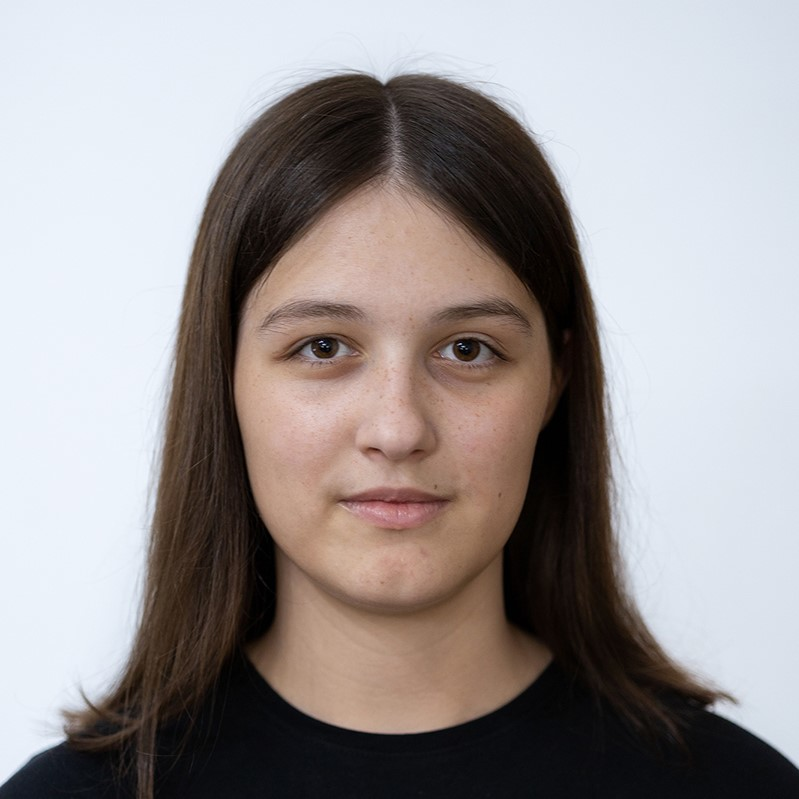
\includegraphics[width=3.5cm]{res/cover/A104437.png} &
            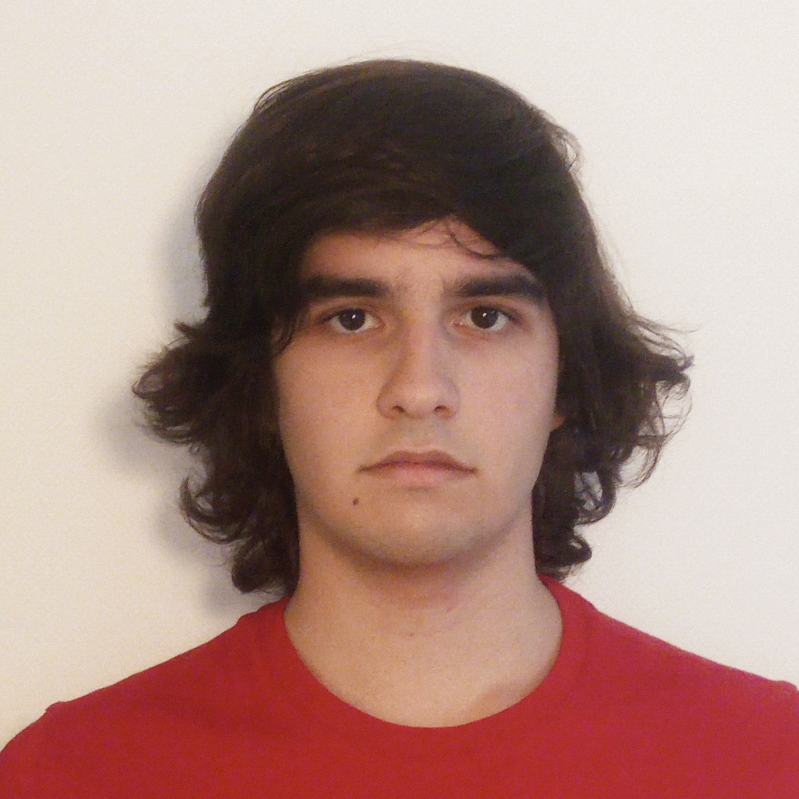
\includegraphics[width=3.5cm]{res/cover/A104348.png} &
            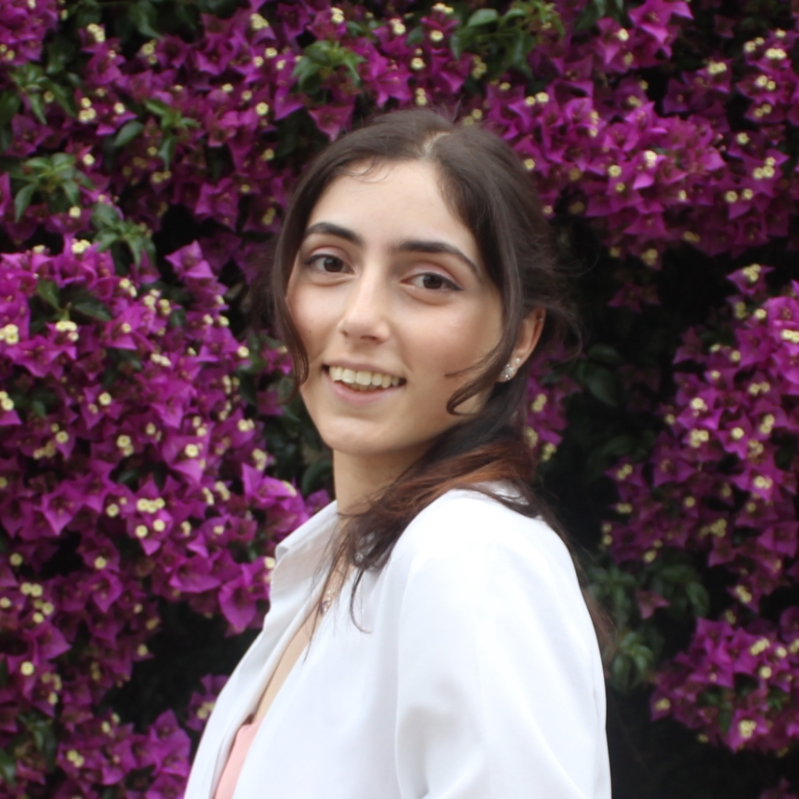
\includegraphics[width=3.5cm]{res/cover/A90817.png} &
            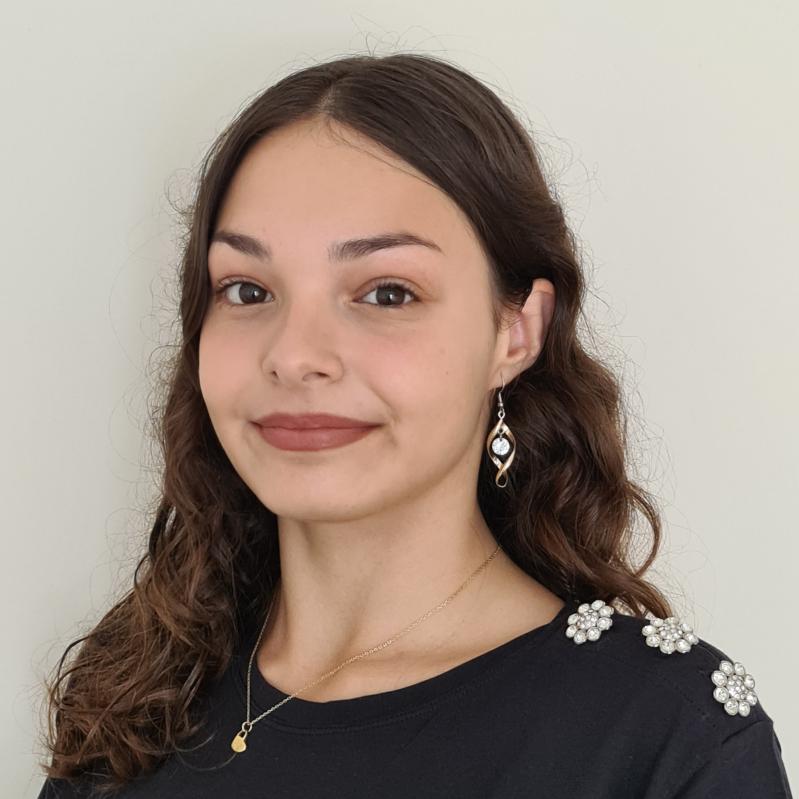
\includegraphics[width=3.5cm]{res/cover/A104179.png} \\

            Ana Oliveira & Humberto Gomes & Mariana Cristino & Sara Lopes \\
            A104437      & A104348        & A90817           & A104179
        \end{tabular}
    \end{center}
\end{adjustwidth}

\pagebreak

\begin{abstract}
    \textbf{\color{red} TODO - resumo}
\end{abstract}

\section{Engine}

\subsection{Câmara Livre}

A câmara livre permite que o utilizador se desloque de forma intuitiva, sendo semelhante à de
jogos de exploração na primeira pessoa, como simuladores de voo, e ambientes de realidade
virtual.
De seguida, descrevem-se os diferentes tipos de movimento suportados.

\subsubsection{Movimentação}

A câmara pode deslocar-se e rodar de forma contínua no espaço tridimensional, sendo os seus
movimentos definidos pelos seguintes vetores diretores:

\begin{itemize}
    \item \textbf{Vetor} $\vec d$: Direção do olhar da câmara.
    \item \textbf{Vetor} $\vec r$: Direção perpendicular ao vetor $\vec d$, ao
          longo do plano horizontal.
    \item \textbf{Vetor} $\mathbf{up}$: Direção vertical da câmara.
\end{itemize}

A posição da câmara é atualizada de acordo com a seguinte equação:

\[
\text{posição} \gets \text{posição} + \text{velocidade} \times \text{direção}
\]

onde a direção depende do movimento escolhido pelo utilizador:

\begin{itemize}
    \item \textbf{Translação horizontal}: O movimento para a frente e para trás ocorre ao longo
          do vetor $\mathbf{front}$, enquanto o movimento lateral ocorre ao longo do vetor
          $\mathbf{right}$.
    \item \textbf{Translação vertical}: O movimento vertical acontece ao longo do vetor
          $\mathbf{up}$, permitindo ao utilizador subir e descer.
    \item \textbf{Rotação}: A orientação da câmara é definida pelos ângulos $\mathbf{yaw}$
          (rotação horizontal) e $\mathbf{pitch}$ (inclinação vertical), que determinam a direção
          do vetor $\mathbf{front}$.
\end{itemize}

\subsubsection{Atualização da Direção da Câmara}

A atualização da orientação da câmara obtém-se através da conversão dos ângulos $\mathbf{yaw}$ e
$\mathbf{pitch}$ para um vetor de direção tridimensional. A relação entre os ângulos e os
componentes do vetor $\mathbf{front}$ é dada por:

\[
\begin{aligned}
    \text{front}_x &= \cos(\text{pitch}) \cdot \cos(\text{yaw}) \\
    \text{front}_y &= \sin(\text{pitch}) \\
    \text{front}_z &= \cos(\text{pitch}) \cdot \sin(\text{yaw})
\end{aligned}
\]

Após serem calculados os componentes do vetor, este é normalizado, uma vez que é necessário
garantir que este mantém um comprimento unitário:

\[
\mathbf{front} \gets \frac{\mathbf{front}}{||\mathbf{front}||}
\]

Esta normalização é fundamental para garantir que a câmara mantém uma velocidade constante em
qualquer direção.

Além disso, foram tomadas medidas para prevenir o $\mathbf{gimbal}$  $\mathbf{lock}$.
Este é um problema que ocorre quando dois eixos de rotação se alinham, reduzindo
os graus de liberdade da rotação. No contexto da câmara livre desenvolvida, este problema surge
quando $\mathbf{pitch}$ antinge um dos seus limites superiror ou inferior, quando o vetor
$\mathbf{front}$ se alinha com o eixo vertical $\mathbf{up}$, o que impossibilita a rotação
horizontal ($\mathbf{yaw}$). Para evitar esta situação, é imposto um limite a $\mathbf{pitch}$:

\[
-89^\circ \leq \mathbf{pitch} \leq 89^\circ
\]

Isto impede que a câmara olhe completamente para cima ou para baixo, garantindo que o vetor
$\mathbf{up}$ mantém uma orientação bem definida e evitando a perda de controlo sobre a rotação
horizontal.

O novo ponto de destino da câmara ($\mathbf{lookAt}$) é atualizado através da soma do vetor
normalizado e da posição atual:

\[
\mathbf{lookAt} = \text{\textbf{posição}} + \mathbf{front}
\]

Além disso, os vetores $\mathbf{right}$ e $\mathbf{up}$ são recalculados para garantir que a
orientação da câmara permanece coerente. O vetor $\mathbf{right}$ é obtido como o produto
vetorial entre um vetor de referência vertical $(0,1,0)$ e o vetor $\mathbf{front}$:

\[
\mathbf{right} = \mathbf{front} \times (0,1,0)
\]

Por fim, o vetor $\mathbf{up}$ é recalculado para ser ortogonal aos outros dois vetores:

\[
\mathbf{up} = \mathbf{right} \times \mathbf{front}
\]

Isto assegura que os movimentos laterais, verticais e de rotação permanecem coerentes em
qualquer orientação da câmara, garantindo um comportamento previsível para o utilizador.

\subsubsection{Controlo por parte do utilizador}

O utilizador pode controlar a câmara de forma intuitiva, utilizando o teclado para movimentação
e as setas direcionais para rotação:

\begin{itemize}
    \item \textbf{W/S:} Movem a câmara para a frente/trás.
    \item \textbf{A/D:} Movem a câmara para os lados.
    \item \textbf{Espaço (SPACE):} Sobe a câmara.
    \item \textbf{Shift Esquerdo (LEFT SHIFT):} Desce a câmara.
    \item \textbf{Seta Esquerda/Direita:} Roda a câmara para a esquerda/direita.
    \item \textbf{Seta Cima/Baixo:} Inclina a câmara para cima/baixo.
\end{itemize}

\section{Transformações}

\textbf{\color{red} TODO - transformações}

\section{Modelo estático do sistema solar}

\textbf{\color{red} TODO - sistema solar}

\section{Extras}

\textbf{\color{red} TODO - extras}

\section{Resultados obtidos}

\textbf{\color{red} TODO - resultados}

\section{Conclusão e Trabalho Futuro}

\textbf{\color{red} TODO - conclusão}

\begingroup
\section{Bibliografia}
\renewcommand{\section}[2]{}

\begin{thebibliography}{9}
    \bibitem{exemplo}
        \href{https://youtu.be/dQw4w9WgXcQ}{Um item de exemplo na bibliografia}
\end{thebibliography}
\endgroup

\end{document}
